% !TEX root = ../Main.tex
\subsection{Freidberg's simple reactor model}
In the \nth{5} chapter of the textbook by Freidberg\cite{freidberg_plasma_2007}, he makes a simple model for designing a fusion reactor power plant.
The model uses simple geometric and electromagnetic assumptions with little involvement of plasma physics. The variables put into the model are shown in \cref{VFR}.
\begin{table}
	\begin{tabular}{lr}
		\toprule
		Symbol                         & Quantity                                                                                 \\
		\midrule
		\(n_\mathrm{flux \ fraction}\) & n flux in breeder end/n flux in breeder start \(\bqty{}\)                                \\
		\(C_F\)                        & Fixed cost propotionality constant \(\bqty{\$}\)                                         \\
		\(C_I\)                        & Nuclear island cost propotionality constant \(\bqty{\$\cdot\si{\watt\per\meter\cubed}}\) \\
		\(P_E\)                        & Desired output power \(\bqty{\si{\mega\watt}}\)                                          \\
		\(P_W\)                        & Maximum wall load \(\bqty{\si{\mega\watt\per\meter\squared}}\)                           \\
		\(B_{\max}\)                   & Magnetic field at the edge of the coil \(\bqty{\si{\tesla}}\)                            \\
		\(\sigma_{\max}\)              & Tensile strenght of the magnetic field coils \(\bqty{\si{\atm}}\)                        \\
		\(\eta_t\)                     & Energy conversion efficiency \(\bqty{}\)                                                 \\
		\bottomrule
	\end{tabular}
	\caption{Variables in the Freidberg's model}
	\label{VFR}
\end{table}
\cref{QFR} shows the output quantities from the model.
\begin{table}
	\begin{tabular}{llr}
		\toprule
		Symbol                    & Quantity                                                       & Obtained values                  \\
		\midrule
		\(b\)                     & Blanket-and-shield thickness                                   & \SI{1.2037}{\meter}              \\
		\(c\)                     & Magnet coil thickness                                          & \SI{0.7993}{\meter}              \\
		\(a\)                     & Minor radius                                                   & \SI{2.0098}{\meter}              \\
		\(R_0\)                   & Major radius                                                   & \SI{4.9583}{\meter}              \\
		\(A\)                     & Aspect ratio                                                   & 2.4670                           \\
		\(A_p\)                   & Plasma surface                                                 & \SI{393.4152}{\meter\squared}    \\
		\(V_p\)                   & Plasma volume                                                  & \SI{395.3509}{\meter\cubed}      \\
		\(P_\mathrm{dens}\)       & Power density                                                  & \SI{4.9685e06}{\watt\per\meter}  \\
		\(p\)                     & Plasma pressure                                                & \SI{7.3672e05}{\pascal}          \\
		\(n\)                     & Particle density                                               & \SI{1.5327e20}{\per\meter\cubed} \\
		\(B_0\)                   & Magnetic field at magnetic axis                                & \SI{4.5744}{\tesla}              \\
		\(\beta\)                 & Normalised plasma pressure                                     & 8.85\%                           \\
		\(\tau_{E_\mathrm{min}}\) & Min confinement time for \(\pqty{p\times\tau_E}_\mathrm{min}\) & \SI{1.1415}{\second}             \\
		\bottomrule
	\end{tabular}
	\caption{Output quantities in the model in Freidberg's\cite{freidberg_plasma_2007} along with the obtained values when inserting the parameters from \cref{Inputparam}}
	\label{QFR}
\end{table}
This model has been implemented in a matlab script provided for the course. The script is shown included in \cref{tokamakDTU_asign_1}.
As an example, the model is run with the following parameters:
\begin{alignat}{3}
	n_\mathrm{flux \ fraction} & = 0.01                                 & \quad P_E      & = \SI{1000}{\mega\watt} \nonumber       \\
	P_W                        & = \SI{4}{\mega\watt\per\meter\squared} & \quad B_{\max} & = \SI{13}{\tesla}    \label{Inputparam} \\
	\sigma_{\max}              & = \SI{3000}{\atm}                      & \quad \eta_t   & = 0.4 \nonumber
\end{alignat}
Note that \(C_F\) and \(C_I\) has been ommited as these serve no purpose for this assignment. It is not of interest how expensive the plant will be. Rather the geometries and physical quantities are of interest.
The results from the model is given in \cref{QFR}.
\subsection{Model sensitivity}
At this point Freidberg has provided a model that produce some reasonable results for a powerplant. It could be interesting to see how this model behaves when some vital parameters are changed. In the last section the model used the parameters shown in \cref{Inputparam}. Now the model will be iteratet over variations in the following parameters, while retaining the rest.
The variable parameters are the electric power \(P_E\), the maximum wall loading \(P_W\), the maximum magnetic field \(B_{\max}\) and the maximum stress \(\sigma_{\max}\).
\cref{IterateTokamakDTU} includes the code for iterating the matlab model over various paremeters.
\subsubsection{Change in desired power output.}
For the rise in megawatts produced (\SIrange{500}{1000}{\mega\watt}) there are a linear rise in aspect ratio, major radius, plasma surface and plasma volume. The rest of the parameters where constant except for the magnetic field strenght at the magnetic axis and the normalised plasma pressure. These are shown in \cref{PE}.
\begin{figure}
	\centering
	\begin{subfigure}[b]{.45\textwidth}
		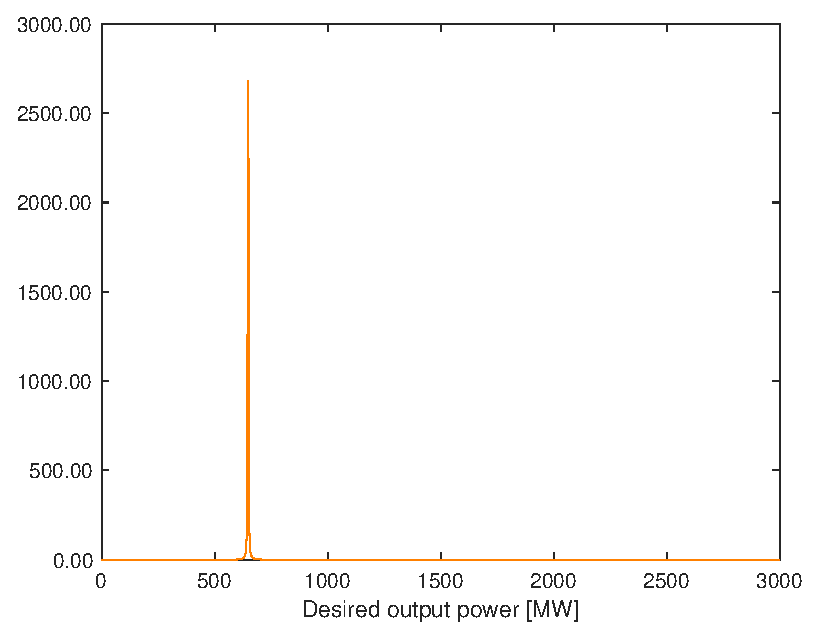
\includegraphics[width=\textwidth]{MatlabFigures/DesiredOutputPower/PlasmaBetaInTheCentre.eps}
		\caption{}
		\label{PEbeta}
	\end{subfigure}
	~
	\begin{subfigure}[b]{.45\textwidth}
		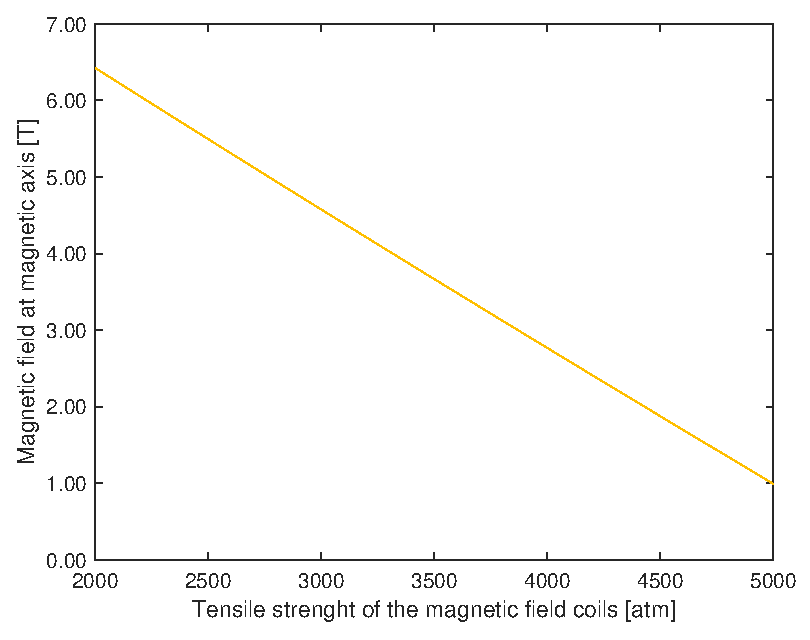
\includegraphics[width=\textwidth]{MatlabFigures/DesiredOutputPower/MagneticFieldAtMagneticAxis.eps}
		\caption{}
		\label{PEmagnet}
	\end{subfigure}
	\caption{The evolution of the normalised plasma pressure (\cref{PEbeta}) and the magnetic field strenght (\cref{PEmagnet}) when changing the desired power output.}
	\label{PE}
\end{figure}
% \subsubsection{\(P_W\) \SIrange{0}{10}{\mega\watt\per\meter\squared}}
% \subsubsection{\(B_{\max}\) \SIrange{0}{20}{\tesla}}
% \subsubsection{\(\sigma_{\max}\) \SIrange{2000}{5000}{\atm}}
\subsection{Elliptic Cross section}
Freidberg's model assumes a circular cross section of the plasma. In reality this is not the case, and as of such we will now make a more realistic, yet still approximate reactor for an elliptic plasma cross section.
In describing the geometry one refers to the elongation ratio:
\begin{align}
	\kappa = \frac{a_{\max}}{a_{\min}}
\end{align}
This parameter ensure a true epilliptic cross section as defined by the equation,
\begin{align}
	\frac{x^2}{a_{\max}}+\frac{y^2}{a_{\min}} = 1
\end{align}
, even after increasing the radii to accomodate the larger ellipses describing the blanket-and-shield. This does however mean that the fixed thickness, \(b\) from Freidberg's model is variable. To find this variation the parametric ellipses defining the blanket-and-shield are defined with \(b\) being the length difference between the larger radii and the length deifference between the smaller radii.
\begin{wrapfigure}[14]{r}{.4\textwidth}
	%\vspace{-5mm}
	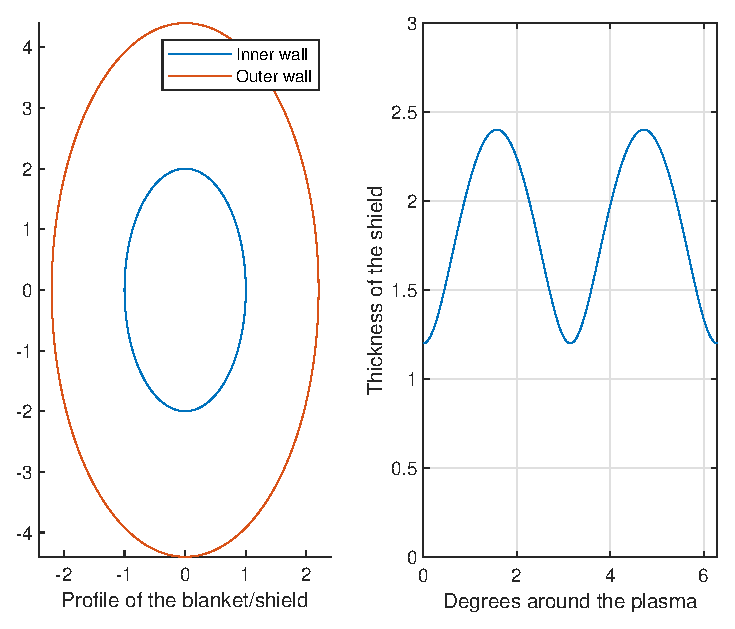
\includegraphics[width=.4\textwidth]{MatlabFigures/ShieldThickness/ShieldThickness.eps}
	\caption{The profile of the blanket-and-shield and the thickness as a function of the angle around origo, \(\phi\). The parameters here are given in \cref{ellparam}}
	\label{ShTh}
\end{wrapfigure}
\begin{align}
	\mqty[x_1 \\y_1] &= \mqty[a_{\min}\cos{\phi}\\\kappa a_{\min}\sin{\phi}] \\
	\mqty[x_2 \\y_2] &= \mqty[\pqty{b+a_{\min}}\cos{\phi}\\\kappa \pqty{b+a_{\min}}\sin{\phi}]
\end{align}
At a given angle, \(\phi\), the distance must be:
\begin{align}
	\vb{u}-\vb{v}       & = \mqty[\cos{\phi}b                                  \\\kappa\sin{\phi}b] \\
	\abs{\vb{u}-\vb{v}} & = \sqrt{\cos^2{\phi}\ b^2+\kappa^2\sin^2{\phi}\ b^2}
\end{align}
An example is given in \cref{ShTh}. Here the parameters are:
\begin{alignat}{3}\label{ellparam}
	\mqty{a_{\min} \\\kappa\\b}&\ \mqty{=\\=\\=}\ &\mqty{2\\2\\1.2}
\end{alignat}
